\documentclass[conference]{IEEEtran}
\IEEEoverridecommandlockouts
% The preceding line is only needed to identify funding in the first footnote. If that is unneeded, please comment it out.
%Template version as of 6/27/2024

\usepackage{cite}
\usepackage{amsmath,amssymb,amsfonts}
\usepackage{algorithm}
\usepackage{algorithmic}
\usepackage{graphicx}
\usepackage{textcomp}
\usepackage[hidelinks]{hyperref}
\usepackage{xcolor}
\usepackage{tikz}
\usetikzlibrary{arrows.meta,calc,positioning,shapes.geometric}
\def\BibTeX{{\rm B\kern-.05em{\sc i\kern-.025em b}\kern-.08em
    T\kern-.1667em\lower.7ex\hbox{E}\kern-.125emX}}
\begin{document}

\title{\fontsize{22}{26}\selectfont
The Price of Location Privacy: Age of Incorrect\\
Information in Location-Aided UAV Communications}

% Draft placeholder; replace with the actual author list before submission.
\author{\IEEEauthorblockN{Author information to be added}}

\maketitle

\begin{abstract}
Location information increasingly supports wireless resource allocation through location-aided channel prediction and beam selection. Protecting this information can affect transmission reliability and the delivery of correct task updates. We consider a single-antenna unmanned aerial vehicle (UAV) communicating with a multi-antenna base station. The UAV releases a three-dimensional Laplace-perturbed location, and the base station applies maximum a posteriori (MAP) inference before selecting a receive beam. For a prescribed beam map and symmetric binary task source, we relate privacy-dependent outage to average age of incorrect information (AoII). Location-Aware Privacy--Information Selection (LAPIS) selects a fixed reporting budget using simultaneous confidence bounds and independent confirmation. In a conditional empirical model constructed from measured channel state information (CSI), MAP lookup yields an estimated 15.8\% lower AoII than direct-report lookup at one tested budget. With 200 selection samples per scenario and budget, point-estimate selection violates the AoII constraint in 65.7\% of 1,000 trials, whereas LAPIS has no observed violations and selects larger disclosure budgets. Separate geometric controls show that larger arrays can increase sensitivity to location uncertainty. These results quantify a privacy--reliability tradeoff under explicit model assumptions. Code and reproducibility materials: \url{https://github.com/jwentong/LocationPrivacy}.
\end{abstract}

\begin{IEEEkeywords}
Location privacy, geo-indistinguishability, location-aided beamforming, age of incorrect information, UAV communications.
\end{IEEEkeywords}

\section{Introduction}
\label{sec:introduction}
Spatial intelligence is creating demand for networks that understand where devices operate and how their surroundings affect communication~\cite{wang2026spatial}. This is particularly relevant to the low-altitude economy, where unmanned aerial vehicle (UAV) applications require reliable links for sensing, inspection, and logistics in three-dimensional environments~\cite{jiang2023lae}. Location consequently becomes more than a navigation coordinate: it links a terminal to environmental knowledge and can guide wireless resource allocation.

Existing research provides several enabling components. Location-based beamforming learns resource decisions from spatial information, including in non-line-of-sight environments~\cite{lemagoarou2022location}. Neural radio-frequency radiance fields (NeRF$^2$) model radio propagation through a continuous field conditioned on transmitter location~\cite{zhao2023nerf2}. Wireless radiation field reconstruction with Gaussian splatting (WRF-GS) reconstructs spatial spectra using three-dimensional Gaussian splatting~\cite{wen2025wrfgs}, while WRF-GS+ improves field representation and prediction~\cite{wen2026wrfgsplus}. These advances support reusable environmental models and can reduce repeated channel acquisition. Their resource decisions nevertheless depend on the quality of the reported location.

Such uncertainty arises naturally from privacy protection. Accurate location reports expose a device's whereabouts and activities. Geo-indistinguishability protects reports through distance-based differential privacy~\cite{andres2013geo}, including three-dimensional mechanisms~\cite{min2022three}. Related work protects against physical-layer localization using transmit beamforming~\cite{checa2020privacy}, studies age of information (AoI) with privacy-aware mobile agents~\cite{jin2021privacy}, and mitigates location leakage in federated radio-map construction~\cite{tian2025geometry}. We examine their operational consequence: how does protecting the location used for resource decisions affect subsequent task-information updates?

Consider a UAV whose location report is used by a multi-antenna base station (BS) to configure a receive beam. Stronger protection can increase inference error and beam mismatch. Radial and angular location errors affect array gain differently, while the link margin determines whether a gain loss causes an outage. Task evolution further determines whether missed packets leave the receiver with an incorrect estimate. Age of incorrect information (AoII) measures how long that estimate remains incorrect~\cite{maatouk2020aoii}. Studies of imperfect channel information~\cite{chen2021imperfect} and low-altitude multiple-input multiple-output (MIMO) networks~\cite{chen2025air} motivate connecting resource errors to persistent information errors.

\begin{figure*}[t]
\centering
\resizebox{\textwidth}{!}{% Editable vector diagram. Coordinates below are layout coordinates, not metres.
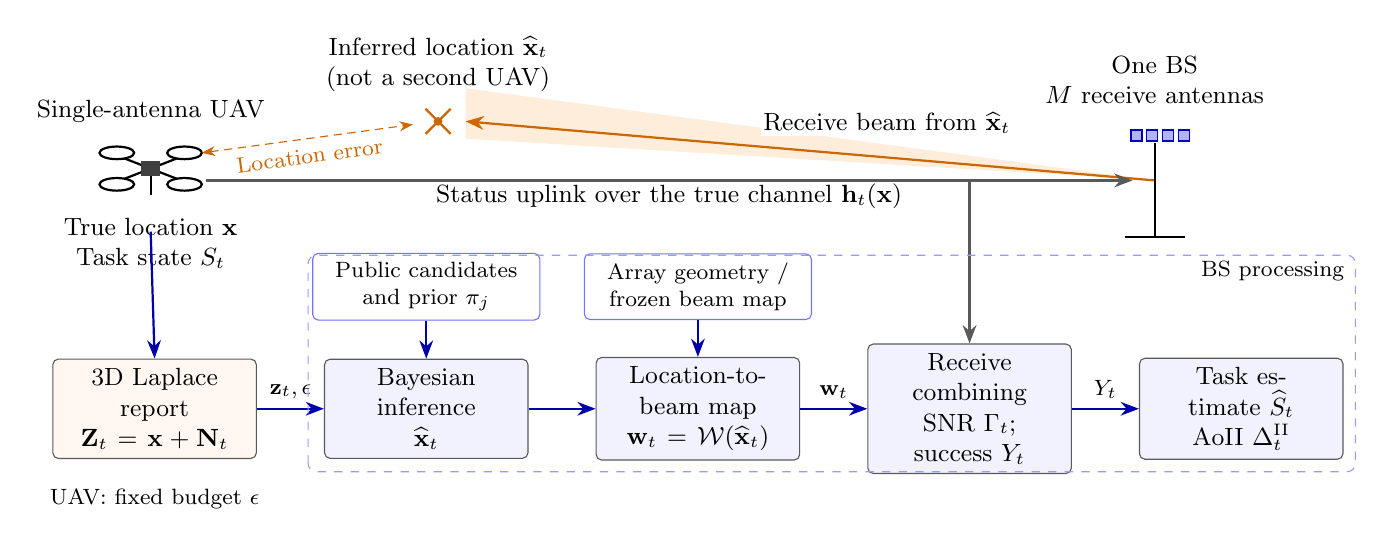
\begin{tikzpicture}[x=1cm,y=1cm,>=Stealth,
  block/.style={draw=black!65,rounded corners=2pt,fill=blue!5,
    minimum height=1.05cm,text width=2.35cm,align=center,font=\small},
  flow/.style={->,thick,draw=blue!65!black},
  lab/.style={font=\small,align=center}]
% One physical UAV and one BS; the orange point is an inferred location.
\begin{scope}[shift={(1.35,3.5)}]
  \draw[thick] (-.36,-.14)--(.36,.14) (-.36,.14)--(.36,-.14);
  \foreach \x/\y in {-.43/-.2,-.43/.2,.43/-.2,.43/.2}
    \draw[thick,fill=white] (\x,\y) ellipse (.22 and .08);
  \fill[black!75] (-.12,-.1) rectangle (.12,.1);
  \draw[thick] (0,-.1)--(0,-.34);
  \node[lab,anchor=south] at (0,.46) {Single-antenna UAV};
  \node[lab,anchor=north] at (0,-.5) {True location $\mathbf x$\\Task state $S_t$};
\end{scope}
\fill[orange!80!black] (5.0,4.1) circle (.055);
\draw[orange!80!black,thick] (4.84,3.94)--(5.16,4.26)
  (4.84,4.26)--(5.16,3.94);
\node[lab,anchor=south] at (5.0,4.35)
  {Inferred location $\widehat{\mathbf x}_t$\\(not a second UAV)};
\draw[<->,orange!80!black,densely dashed] (2.0,3.7)--(4.68,4.06)
  node[midway,below,font=\footnotesize,sloped] {Location error};
% Illustrative mismatched receive beam and the true propagation direction.
\fill[orange!14] (14.1,3.35)--(5.35,4.52)--(5.35,3.88)--cycle;
\draw[orange!80!black,thick,->] (14.1,3.35)--(5.35,4.1);
\node[lab,fill=white,inner sep=1pt] at (10.7,4.08)
  {Receive beam from $\widehat{\mathbf x}_t$};
\draw[->,thick,draw=black!65] (2.05,3.35)--(13.82,3.35)
  node[midway,below,fill=white,inner sep=1pt,font=\small]
  {Status uplink over the true channel $\mathbf h_t(\mathbf x)$};
\begin{scope}[shift={(14.1,3.35)}]
  \draw[thick] (0,-.7)--(0,.48);
  \draw[thick] (-.38,-.72)--(.38,-.72);
  \foreach \x in {-.3,-.1,.1,.3}
    \draw[fill=blue!30,draw=blue!70!black] (\x,.5) rectangle +( .14,.14);
  \node[lab,anchor=south] at (0,.85) {One BS\\$M$ receive antennas};
\end{scope}
% Report, decision, and decoding paths.
\node[block,fill=orange!6] (dp) at (1.4,.45)
  {3D Laplace report\\$\mathbf Z_t=\mathbf x+\mathbf N_t$};
\node[block] (map) at (4.85,.45)
  {Bayesian inference\\$\widehat{\mathbf x}_t$};
\node[block] (beam) at (8.3,.45)
  {Location-to-beam map\\$\mathbf w_t=\mathcal W(\widehat{\mathbf x}_t)$};
\node[block] (rx) at (11.75,.45)
  {Receive combining\\SNR $\Gamma_t$; success $Y_t$};
\node[block] (age) at (15.2,.45)
  {Task estimate $\widehat S_t$\\AoII $\Delta_t^{\rm II}$};
\draw[flow] (dp)--(map) node[midway,above,font=\footnotesize] {$\mathbf z_t,\epsilon$};
\draw[flow] (map)--(beam);
\draw[flow] (beam)--(rx) node[midway,above,font=\footnotesize] {$\mathbf w_t$};
\draw[flow] (rx)--(age) node[midway,above,font=\footnotesize] {$Y_t$};
\draw[flow] (1.35,2.7)--(dp.north);
\node[draw=blue!55,fill=white,rounded corners=2pt,font=\footnotesize,
  align=center,text width=2.65cm] (prior) at (4.85,2.0)
  {Public candidates\\and prior $\pi_j$};
\draw[flow] (prior)--(map);
\node[draw=blue!55,fill=white,rounded corners=2pt,font=\footnotesize,
  align=center,text width=2.65cm] (field) at (8.3,2.0)
  {Array geometry /\\frozen beam map};
\draw[flow] (field)--(beam);
\draw[flow,draw=black!65] (13.35,3.35)--(11.75,3.35)--(rx.north);
\draw[draw=blue!40,dashed,rounded corners=3pt]
  (3.35,-.35) rectangle (16.65,2.4);
\node[font=\footnotesize,anchor=north east,fill=white,inner sep=1pt]
  at (16.55,2.36) {BS processing};
\node[font=\footnotesize,anchor=north] at (1.4,-.45)
  {UAV: fixed budget $\epsilon$};
\end{tikzpicture}
}
\caption{Location-private UAV uplink. A perturbed report drives inference and receive-beam selection. The green ellipse represents a receive beam directed toward the inferred location (orange target), while the task packet traverses the channel at the true location.}
\label{fig:system}
\end{figure*}
We study this connection in a single-UAV uplink with one transmit antenna and multiple BS receive antennas. A three-dimensional Laplace mechanism protects reports; maximum a posteriori (MAP) inference determines a location-aided receive beam, which is evaluated on the true channel. A separate Markovian task source connects link outcomes to AoII. We protect the report interface and assume the controller has no independent precise radio-frequency (RF) localization. The challenge is to quantify the coupled effects of privacy, inference, directional gain, outage, and source evolution. The contributions are:
\begin{itemize}
\item A model connecting three-dimensional report privacy and Bayesian inference to receive-beam decisions and actual transmission outage.
\item An analysis that specializes established binary-source AoII models to location-dependent outages, capturing the occurrence and persistence of incorrect task estimates.
\item Location-Aware Privacy--Information Selection (LAPIS), a finite-grid procedure combining established concentration bounds with independent confirmation under privacy or AoII requirements.
\end{itemize}
Experiments using measured channel state information (CSI) and geometric controls quantify the tradeoff. At one tested budget, MAP lookup yields an estimated 15.8\% lower AoII. With 200 selection samples per scenario and budget, point-estimate selection violates the AoII constraint in 65.7\% of 1,000 trials, versus no observed violations for LAPIS, which selects larger disclosure budgets (Section~\ref{sec:results}).

\section{System Model}
\label{sec:system}
\subsection{Network and Update Protocol}
In Fig.~\ref{fig:system}, a single-antenna UAV communicates with a BS at $\mathbf b\in\mathbb R^3$ using an $M_x\times M_y$ uniform planar array (UPA), $M=M_xM_y$. The UAV hovers at $\mathbf x\in\mathcal X\subset\mathbb R^3\setminus\{\mathbf b\}$ per session; locations define separate scenarios. Power $P$, array, and packet requirements are fixed across budgets.

Each slot lasts $T$. At its start, the UAV generates state $S_t$ and a noisy location report. A reliable control path delivers the report before beam configuration and state-packet transmission. The state remains constant within the slot; reception is assessed at its end. Failed packets are discarded. Fixed control overhead leaves data duration $\tau_d$, identically across budgets.

The controller selects beams using reports, the public prior, and a frozen map. Its observations exclude independent precise localization and full instantaneous array CSI. The privacy guarantee covers reports; RF localization requires a separate threat model. Task states are independent of location and channel randomness.


\subsection{Private Location Reporting and Inference}
For a fixed budget $\epsilon>0$, the UAV releases $\mathbf Z_t=\mathbf x+\mathbf N_t$, independently each slot. Following geo-indistinguishability~\cite{andres2013geo,min2022three}, we use the three-dimensional isotropic Laplace density
\begin{equation}
 f_\epsilon(\mathbf z\mid\mathbf x)
 =\frac{\epsilon^3}{8\pi}\exp(-\epsilon\|\mathbf z-\mathbf x\|_2).
 \label{eq:laplace}
\end{equation}
The triangle inequality gives
\begin{equation}
 f_\epsilon(\mathbf z\mid\mathbf x)
 \le e^{\epsilon\|\mathbf x-\mathbf x'\|_2}
 f_\epsilon(\mathbf z\mid\mathbf x').
 \label{eq:gi}
\end{equation}
Thus $\eta=\epsilon r_0$ is the dimensionless single-report budget within a protection distance $r_0$; smaller $\eta$ provides stronger protection. Here $\epsilon$ has units $\mathrm m^{-1}$. Reports retain their full spatial support. The noise radius satisfies $\|\mathbf N_t\|_2\sim\mathrm{Gamma}(3,1/\epsilon)$ in shape--scale notation, with mean $3/\epsilon$. 

Let $\mathcal X=\{\mathbf x_j\}_{j=1}^{N_{\mathrm x}}$, with $N_{\mathrm x}=|\mathcal X|$, be a public candidate set with fixed prior probabilities $\pi_j>0$, $\sum_j\pi_j=1$. A report $\mathbf z_t$ yields posterior
\begin{equation}
 \rho_t(j)=
 \frac{\pi_j e^{-\epsilon\|\mathbf z_t-\mathbf x_j\|_2}}
 {\sum_{k=1}^{N_{\mathrm x}}\pi_k e^{-\epsilon\|\mathbf z_t-\mathbf x_k\|_2}},
 \quad
 \widehat{\mathbf x}_t=\mathbf x_{\arg\max_j\rho_t(j)}.
 \label{eq:map}
\end{equation}
Ties use a fixed rule. The prior and candidate set are public and fixed before reporting. The prescribed receiver applies current-report MAP; optimal attacks, AoII-optimal beam selection, and temporal filtering remain outside the scope. Post-processing preserves~\eqref{eq:gi}. For $K$ retained reports, the likelihood ratio is bounded by $e^{K\epsilon\|\mathbf x-\mathbf x'\|_2}$, which quantifies the cumulative privacy loss across the session.

\subsection{Location-Aided Receive Beamforming}
We adapt location-to-beam mapping~\cite{lemagoarou2022location} to uplink combining. For wavelength $\lambda_c$ and array-relative element locations $\mathbf r_m$, the far-field narrowband steering vector for $\mathbf v\ne\mathbf b$ is
\begin{equation}
 \mathbf u(\mathbf v)=\frac{\mathbf v-\mathbf b}{\|\mathbf v-\mathbf b\|_2},
 \qquad
 [\mathbf a(\mathbf v)]_m
 =e^{\mathrm j(2\pi/\lambda_c)\mathbf r_m^{\mathsf T}\mathbf u(\mathbf v)}.
 \label{eq:array}
\end{equation}
For a UPA, $\mathbf r_{m_x,m_y}=(m_xd_x,m_yd_y,0)^{\mathsf T}$, where $0\le m_x<M_x$ and $0\le m_y<M_y$, and all coordinates share the array frame. Hence $\|\mathbf a(\mathbf v)\|_2^2=M$. A Rician baseline is
\begin{equation}
 \mathbf h_t(\mathbf x)=\sqrt{\beta(\mathbf x)}
 \left(\sqrt{\frac{\kappa}{\kappa+1}}\mathbf a(\mathbf x)
 +\sqrt{\frac{1}{\kappa+1}}\mathbf g_t\right),
 \label{eq:channel}
\end{equation}
where $\mathbf g_t\sim\mathcal{CN}(\mathbf0,\mathbf I_M)$ is independent and identically distributed (i.i.d.) across slots and independent of report noise, $\kappa$ is the linear Rician factor, and $\beta(\mathbf x)=\beta_0(\|\mathbf x-\mathbf b\|_2/d_0)^{-\nu}$ is the single-element large-scale power gain, with $\beta_0,d_0>0$ and $\nu>0$. The line-of-sight (LOS) limit is obtained as $\kappa\to\infty$.

Given a frozen map output $\boldsymbol\psi(\mathbf v)\in\mathbb C^M\setminus\{\mathbf0\}$, the receive beam is
\begin{equation}
 \mathbf w_t=\mathcal W(\widehat{\mathbf x}_t)
 =\frac{\boldsymbol\psi(\widehat{\mathbf x}_t)}
 {\|\boldsymbol\psi(\widehat{\mathbf x}_t)\|_2},
 \qquad \|\mathbf w_t\|_2=1.
 \label{eq:beam}
\end{equation}
The geometric model uses $\boldsymbol\psi(\mathbf v)=\mathbf a(\mathbf v)$; the empirical map uses a covariance eigenvector (Section~\ref{sec:results}). Channel predictions with spatial phase information also support~\eqref{eq:beam}. A fixed unit beam handles zero outputs. The digital beam map permits general complex weights and remains fixed during budget optimization.

For unit-energy data symbol $s_t$ and receiver noise $\mathbf n_t^{\rm RF}\sim\mathcal{CN}(\mathbf0,\sigma^2\mathbf I_M)$, independent of other randomness, the received signal and combined signal-to-noise ratio (SNR) are
\begin{align}
 \mathbf y_t&=\sqrt P\mathbf h_t(\mathbf x)s_t+\mathbf n_t^{\rm RF},\nonumber\\
 \Gamma_t&=\frac{P|\mathbf w_t^{\mathsf H}\mathbf h_t(\mathbf x)|^2}{\sigma^2}.
 \label{eq:snr}
\end{align}
Unit-norm combining leaves noise power $\sigma^2$. In pure LOS with the geometry-based rule, the mismatch factor and resulting SNR are
\begin{align}
 B_t&=\frac{|\mathbf a(\widehat{\mathbf x}_t)^{\mathsf H}
                   \mathbf a(\mathbf x)|^2}{M^2}\in[0,1],\nonumber\\
 \Gamma_t&=\Gamma_{\rm al}B_t,
 \qquad \Gamma_{\rm al}=P\beta(\mathbf x)M/\sigma^2.
 \label{eq:mismatch}
\end{align}


\subsection{Outage and Task-Information Correctness}
With fixed packet length $L$ bits and bandwidth $W$, we use the ideal coding threshold $\gamma_{\rm th}=2^{L/(W\tau_d)}-1>0$. Define
\begin{equation}
 Y_t=\mathbf1\{\Gamma_t\ge\gamma_{\rm th}\},\qquad
 p_\epsilon(\mathbf x)=\Pr(Y_t=1\mid\mathbf x,\epsilon),
 \label{eq:success}
\end{equation}
and $q_\epsilon(\mathbf x)=1-p_\epsilon(\mathbf x)$. Outcomes are i.i.d. conditional on a session location, averaging over report noise and fading. In pure LOS, $p_\epsilon(\mathbf x)=\Pr\{B_t\ge\gamma_{\rm th}/\Gamma_{\rm al}\}$. At $\kappa=0$, isotropic scattering makes an independent unit-norm projection direction-invariant, eliminating this directional privacy cost.

Following binary-source AoII models~\cite{maatouk2020aoii,chen2021imperfect}, let $S_t\in\{0,1\}$ be a symmetric Markov chain with $\Pr(S_t=1-s\mid S_{t-1}=s)=\alpha$ for $s\in\{0,1\}$ and $0<\alpha\le1/2$. Successful packets are decoded correctly; only threshold outage is modeled. At slot end,
\begin{equation}
 \widehat S_t=\begin{cases}
 S_t,&Y_t=1,\\
 \widehat S_{t-1},&Y_t=0.
 \end{cases}
 \label{eq:estimate}
\end{equation}
The linear AoII is $\Delta_t^{\rm II}=TA_t$, where
\begin{equation}
 A_t=\begin{cases}
 0,&S_t=\widehat S_t,\\
 A_{t-1}+1,&S_t\ne\widehat S_t.
 \end{cases}
 \label{eq:aoii}
\end{equation}
Source reversal can restore correctness between successful receptions; this event resets the slot-end AoII.


\section{Problem Formulation}
\label{sec:problem}
\subsection{From Outage to Average AoII}
Specializing the binary-source framework of~\cite{maatouk2020aoii,chen2021imperfect} to our slot-end update convention, write $q=q_\epsilon(\mathbf x)$. Since transmission outcomes are independent of the task source and past slots,~\eqref{eq:estimate}--\eqref{eq:aoii} imply
\begin{align}
 \Pr(A_t=1\mid A_{t-1}=0)&=\alpha q\triangleq\mu_0,\nonumber\\
 \Pr(A_t=a+1\mid A_{t-1}=a)&=(1-\alpha)q\triangleq\mu_1,
 \quad a\ge1.
 \label{eq:age-transitions}
\end{align}
All other transitions return to zero. The stationary probabilities are $\xi_0=(1-\mu_1)/(1-\mu_1+\mu_0)$ and $\xi_a=\xi_0\mu_0\mu_1^{a-1}$ for $a\ge1$. Therefore,
\begin{align}
 \overline\Delta_\epsilon^{\rm II}(\mathbf x)
 &\triangleq\lim_{N\to\infty}\frac1N
       \mathbb E\!\left[\sum_{t=1}^{N}TA_t\mid\mathbf x\right]\nonumber\\
 &=T\frac{\alpha q_\epsilon(\mathbf x)}
 {\left[1-(1-\alpha)q_\epsilon(\mathbf x)\right]
  \left[1-(1-2\alpha)q_\epsilon(\mathbf x)\right]}.
 \label{eq:mean-aoii}
\end{align}
For $0<\alpha\le1/2$,~\eqref{eq:mean-aoii} increases with $q$, and perfect transmission yields zero slot-end AoII. Monotonicity in $\epsilon$ additionally depends on inference and beam selection.
% Float declarations placed early to avoid a trailing figure-only page.
\begin{figure*}[!t]
\centering
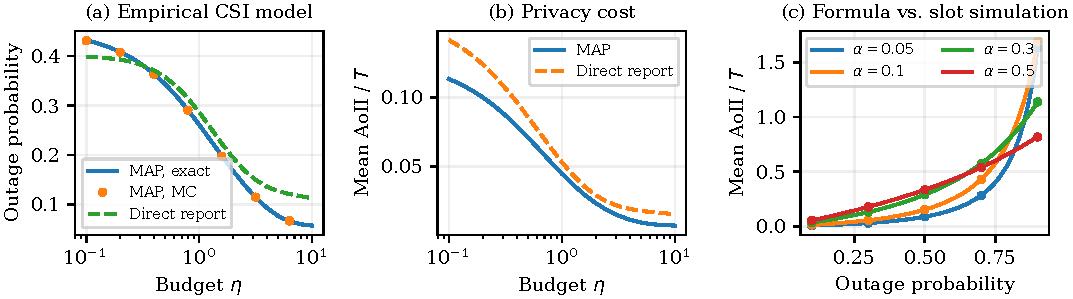
\includegraphics[width=\textwidth]{Figs/mechanism_theory.pdf}
\caption{Empirical-channel privacy cost and analytical validation. Solid MAP curves in (a) use analytical integration; markers and dashed direct-report curves use Monte Carlo (MC). In (c), lines are analytical and markers are direct task-state simulations with nominal pointwise 95\% batch-mean intervals for 36 controlled settings.}
\label{fig:mechanism}
\end{figure*}

\subsection{Fixed Privacy-Budget Selection}
Let $\mathcal E\subset(0,\infty)$ be a finite set of candidate budgets, fixed before testing. To select a common budget for a public distribution of hovering scenarios, specify weights $\omega_j\ge0$, $\sum_j\omega_j=1$, independently of the private test location, and define
\begin{equation}
 J(\epsilon)=\sum_{j=1}^{N_{\mathrm x}}\omega_j
           \overline\Delta_\epsilon^{\rm II}(\mathbf x_j).
 \label{eq:scenario-cost}
\end{equation}
Weights aggregate separate hovering sessions; the MAP prior governs inference within each session. AoII must be averaged after conditioning on location; applying~\eqref{eq:mean-aoii} to average outage generally differs.

Given a maximum single-report budget $\eta_{\max}$ at distance $r_0$, the primary problem is
\begin{equation}
 \begin{aligned}
 \mathrm{(P1)}\quad&\min_{\epsilon\in\mathcal E}&&J(\epsilon)\\
 &\mathrm{subject\ to}&&\epsilon r_0\le\eta_{\max}.
 \end{aligned}
 \label{eq:p1}
\end{equation}
Algorithm~\ref{alg:lapis} selects $\epsilon$ offline for the entire session. Repeated reports accumulate privacy loss across the session. For a finite session of $K$ reports with total budget $B_{\rm priv}$ under the repeated-location model, replace the constraint by $K\epsilon r_0\le B_{\rm priv}$. The selected budget remains fixed throughout the session.

An alternative design perspective prioritizes the strongest report protection compatible with an AoII requirement $D_{\max}$:
\begin{equation}
 \mathrm{(P2)}\quad
 \min_{\epsilon\in\mathcal E}\ \epsilon r_0
 \quad\mathrm{subject\ to}\quad J(\epsilon)\le D_{\max}.
 \label{eq:p2}
\end{equation}
Figure~\ref{fig:mechanism} evaluates the mechanism and AoII mapping. Problems (P1) and (P2) specify alternative requirements. If conditional outages decrease with $\epsilon$, the largest feasible budget solves (P1); no interior optimum is required. Otherwise, candidates are compared under identical link/source conditions, and the selected budget is independently confirmed.




\section{LAPIS: Location-Aware Privacy--Information Selection}
\label{sec:lapis}
Algorithm~\ref{alg:lapis} evaluates a finite grid and selects one fixed reporting budget. The grid, scenarios, prior, beam map, sample counts, and confidence levels are fixed before evaluation; no monotonic outage or convex objective is assumed.

\begin{algorithm}[t]
\caption{LAPIS: Fixed Privacy-Budget Selection}
\label{alg:lapis}
\footnotesize
\begin{algorithmic}[1]
\REQUIRE Public scenarios, prior/weights, grid $\mathcal E$, mode and constraint; $N_s,N_c,\delta_s,\delta_c$.
\ENSURE Fixed $\epsilon^\star$, confirmation interval/status, and (P1) gap $G$; or no candidate.
\STATE Set $\mathcal C=\mathcal E$; for (P1), retain $\epsilon r_0\le\eta_{\max}$.
\STATE If $\mathcal C=\varnothing$, \textbf{return} grid-infeasible.
\STATE Draw i.i.d. report-noise seeds and true-channel samples; reuse across budgets.
\FOR{each $\epsilon\in\mathcal C$}
 \STATE Generate reports; apply MAP and the frozen beam map.
 \STATE Evaluate true-channel outages via~\eqref{eq:success}; estimate $\widehat q_{\epsilon j}$ for each scenario by~\eqref{eq:paired-outage}.
 \STATE Compute $[L_\epsilon,U_\epsilon]$ via~\eqref{eq:outage-confidence}--\eqref{eq:aoii-confidence}.
\ENDFOR
\IF{mode is (P1)}
 \STATE Select $\epsilon^\star$ and compute $G$ by~\eqref{eq:lapis-p1}; ties favor smaller budgets.
\ELSE
 \STATE Set $\mathcal F_D=\{\epsilon\in\mathcal C:U_\epsilon\le D_{\max}\}$.
 \STATE If $\mathcal F_D=\varnothing$, \textbf{return} infeasible when $\min L_\epsilon>D_{\max}$, otherwise unconfirmed; else set $\epsilon^\star=\min\mathcal F_D$.
\ENDIF
\STATE Freeze $\epsilon^\star$; evaluate with $N_c$ new samples per scenario and radius $d_c$ to obtain $[L_c,U_c]$.
\STATE \textbf{return} budget, interval, (P1) privacy status and $G$, or (P2) confirmation iff $U_c\le D_{\max}$; retain the selected budget.
\end{algorithmic}
\end{algorithm}

\subsection{Paired Outage Evaluation}
For each scenario $j$ and sample $\ell$, draw $R_{j\ell}\sim\mathrm{Gamma}(3,1)$, a uniform unit-sphere direction $\mathbf U_{j\ell}$, and independent true-channel samples from~\eqref{eq:channel} or the frozen empirical CSI bank. Reuse these draws across budgets, setting
\begin{align}
 \mathbf z_{j\ell}(\epsilon)
 &=\mathbf x_j+\frac{R_{j\ell}}{\epsilon}\mathbf U_{j\ell},\nonumber\\
 \widehat q_{\epsilon j}
 &=\frac1{N_s}\sum_{\ell=1}^{N_s}(1-Y_{j\ell}(\epsilon)).
 \label{eq:paired-outage}
\end{align}
Each $Y_{j\ell}(\epsilon)$ is computed through~\eqref{eq:map}--\eqref{eq:success} on the same true channel realization. This coupling preserves the marginal distributions and independence across $\ell$. Let $F_\alpha(q)$ denote the right-hand side of~\eqref{eq:mean-aoii}. The plug-in estimate is $\widehat J(\epsilon)=\sum_j\omega_jF_\alpha(\widehat q_{\epsilon j})$.

To account for finite-sample uncertainty, Hoeffding's inequality~\cite{hoeffding1963} and a union bound over $N_{\mathrm x}|\mathcal E|$ pairs give the simultaneous radius
\begin{equation}
 \begin{gathered}
 d_s=\sqrt{\frac{\log(2N_{\mathrm x}|\mathcal E|/\delta_s)}{2N_s}},\\
 q^-_{\epsilon j}=[\widehat q_{\epsilon j}-d_s]_+,\quad
 q^+_{\epsilon j}=\min\{1,\widehat q_{\epsilon j}+d_s\},
 \end{gathered}
 \label{eq:outage-confidence}
\end{equation}
where $[a]_+=\max\{0,a\}$ and $\delta_s\in(0,1)$. Since $F_\alpha$ is increasing, with probability at least $1-\delta_s$, every candidate satisfies
\begin{equation}
 \begin{gathered}
 L_\epsilon=\sum_j\omega_jF_\alpha(q^-_{\epsilon j}),\quad
 U_\epsilon=\sum_j\omega_jF_\alpha(q^+_{\epsilon j}),\\
 L_\epsilon\le J(\epsilon)\le U_\epsilon.
 \end{gathered}
 \label{eq:aoii-confidence}
\end{equation}
These bounds quantify Monte Carlo error conditional on the prescribed map and channel model. Model mismatch requires a separate assessment.

\subsection{Selection and Independent Confirmation}
For (P1), form $\mathcal F_\eta=\{\epsilon\in\mathcal E:\epsilon r_0\le\eta_{\max}\}$ and choose
\begin{equation}
 \begin{gathered}
 \epsilon^\star\in\arg\min_{\epsilon\in\mathcal F_\eta}U_\epsilon,\\
 G=U_{\epsilon^\star}-\min_{\epsilon\in\mathcal F_\eta}L_\epsilon.
 \end{gathered}
 \label{eq:lapis-p1}
\end{equation}
On the simultaneous-coverage event, $J(\epsilon^\star)-\min_{\epsilon\in\mathcal F_\eta}J(\epsilon)\le G$; $G$ bounds unresolved grid suboptimality.

For (P2), choose the smallest $\epsilon$ satisfying $U_\epsilon\le D_{\max}$. If none qualifies, $\min_\epsilon L_\epsilon>D_{\max}$ indicates grid infeasibility on the coverage event; otherwise feasibility is unconfirmed. An interval straddling the threshold leaves grid optimality unresolved.

Freeze the budget and use $N_c$ independent samples per scenario, replacing $d_s$ in~\eqref{eq:outage-confidence}--\eqref{eq:aoii-confidence} by $d_c=\sqrt{\log(2N_{\mathrm x}/\delta_c)/(2N_c)}$. For (P2), confirm feasibility only if the new upper endpoint is at most $D_{\max}$; otherwise report unconfirmed and retain the selected budget. The union-bound coverage for selection and confirmation is at least $1-\delta_s-\delta_c$. For the geometry-based beam rule and brute-force MAP, selection costs $O(|\mathcal E|N_{\mathrm x}N_s(N_{\mathrm x}+M))$, followed by one-candidate confirmation. Figures~\ref{fig:arrays} and~\ref{fig:selection} examine array sensitivity and selection reliability. 

\begin{figure*}[!t]
\centering
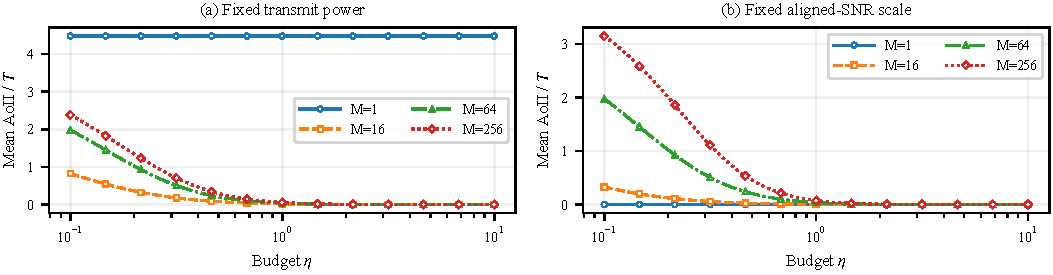
\includegraphics[width=\textwidth]{Figs/array_effect.pdf}
\caption{Geometric Rician array controls. Fixed power uses reference single-element SNR $-5$~dB at 150~m. The second control fixes reference LOS aligned-SNR scale at 13.06~dB, adjusting power as $1/M$.}
\label{fig:arrays}
\end{figure*}
\begin{figure*}[!t]
\centering
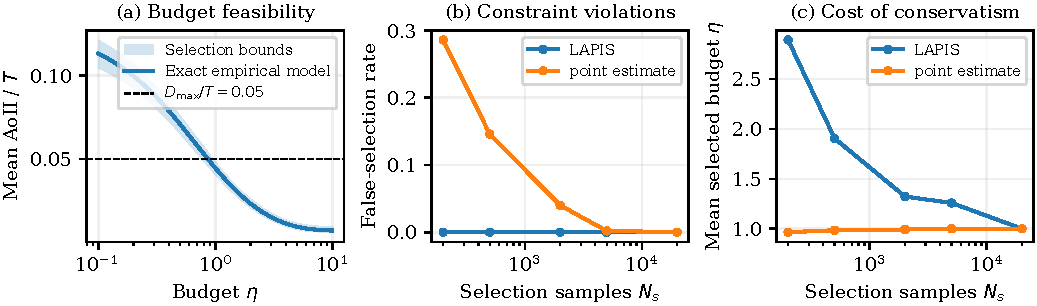
\includegraphics[width=\textwidth]{Figs/selection_reliability.pdf}
\caption{Conditional empirical-model selection. Reliability uses equivalent Bernoulli links, independent budget streams, and 1,000 repetitions at each of 13 sample sizes. Both methods use identical selection samples and grids. Panel (b) reports selections that violate the exact-model constraint; panel (c) shows their disclosure cost.}
\label{fig:selection}
\end{figure*}


\section{Numerical Results}
\label{sec:results}
\subsection{Experimental Setup}
Table~\ref{tab:parameters} gives the settings. One 50-s recording from the MaMIMO-UAV dataset~\cite{colpaert2023dataset} yields 500 location--CSI pairs at 100-ms intervals on one subcarrier. Coverage is $34\times43$~m horizontally, at takeoff-relative heights 25--27.5~m. A 70/30 split of 10-m cells (seed 20261027), with a 2-m guard, retains 287 training and 102 test snapshots and discards 111. Seven covariance eigenvectors form the frozen nearest-cell beam map. Empirical SNR is $10|\mathbf w^{\mathsf H}\mathbf h|^2/\operatorname{median}_{i\in\mathcal T}\|\mathbf h_i\|_2^2$, where $\mathcal T$ contains training snapshots. This configured SNR scale is uncalibrated. Ages and intervals are normalized by $T$, unrelated to measurement spacing.

\begin{table}[t]
\caption{Simulation and Empirical-Channel Settings}
\label{tab:parameters}
\centering
\footnotesize
\setlength{\tabcolsep}{3pt}
\begin{tabular}{p{0.42\columnwidth}p{0.50\columnwidth}}
\hline
Parameter & Value \\
\hline
Privacy distance / budget grid & $r_0=10$~m; 61 log-spaced $\eta\in[0.1,10]$ \\
Default task / threshold & $\alpha=0.1$; $\gamma_{\rm th}=1$; AoII in units of $T$ \\
Empirical receiver / map cells & 64 channels at 2.610~GHz; 10-m cells; 2-m guard \\
Empirical scenarios / weights & Three cell centers; uniform prior and weights \\
Configured empirical SNR scale & 10~dB at median training channel energy \\
Mechanism Monte Carlo samples & $3\times10^5$ per scenario and budget \\
Selection samples (main / sweep) & $2\times10^4$ / 13 sizes, 200--20000 \\
Confirmation samples & $N_c=10^5$ \\
Confidence / macro repetitions & $\delta_s=\delta_c=0.025$; 1,000 repetitions \\
Geometric array control & $M=1,16,64,256$; $d_x=d_y=\lambda_c/2$ \\
Geometric channel / scenarios & $\kappa=10$, $\nu=2$; 75 hovering locations \\
Geometric report samples & $3\times10^4$ per location and budget \\
\hline
\end{tabular}
\end{table}

Three occupied held-out cell centers define the public scenarios before reporting, with 7, 17, and 78 CSI snapshots. Snapshots are independently resampled within cells; scenario weights are equal. The privacy guarantee applies to representative centers, not original Global Positioning System (GPS) coordinates. Collinearity and equal priors permit exact MAP integration. This data-derived grid does not test general three-dimensional map performance. Bounds cover simulation randomness, not measurement representativeness, GPS error, or map mismatch.

\subsection{Privacy Mechanism and AoII Validation}
Figure~\ref{fig:mechanism} traces report privacy through the frozen beam map. Increasing $\eta$ from 0.1 to 10 reduces mean outage from 0.4321 to 0.0571 and normalized AoII from 0.1131 to 0.0072. At $\eta=1$, MAP achieves normalized AoII 0.0446 versus 0.0530 for direct-report map lookup, an estimated 15.8\% reduction. Simultaneous 95\% Monte Carlo bounds for the direct baseline give a relative-reduction interval of [13.9\%, 17.6\%]. MAP need not minimize outage: at $\eta=0.1$, direct lookup has lower mean outage but higher mean AoII. This reflects heterogeneous outages and nonlinear scenario-wise AoII. For 36 controlled source--link settings, $5\times10^6$ simulated slots per setting give maximum relative deviation 0.78\%; nine additional empirical-marginal settings give 1.33\%. These tests assess the i.i.d. mapping, not measured-trajectory AoII.

\subsection{Array Size and Directional Sensitivity}
Figure~\ref{fig:arrays} uses~\eqref{eq:channel} to isolate aperture effects without assuming the measured array's physical ordering. Candidate coordinates are $x,y\in\{-100,-50,0,50,100\}$~m and $z\in\{80,120,160\}$~m; conditional Rician outage is integrated analytically. At fixed power and $\eta=0.1$, AoII rises from 0.821 for $M=16$ to 2.378 for $M=256$, despite the larger aligned gain. At equal reference aligned-SNR scale, the corresponding values are 0.326 and 3.152. Larger arrays therefore do not guarantee better privacy-constrained performance. The $M=1$ curve is budget-independent, as expected. An additional analytical Rayleigh control is direction-independent (not plotted).

\subsection{Budget Selection and Reliability}
For (P1), LAPIS selects the largest feasible grid point for all four tested caps $\eta_{\max}\in\{0.3,1,3,10\}$, matching the exact grid reference. These are boundary optima. For (P2) with $D_{\max}/T=0.05$, it selects $\eta=1$ and independently confirms normalized AoII in $[0.0431,0.0459]$. At the tighter requirement 0.03, it selects $\eta=1.848$, whereas the smallest feasible budget under the exact conditional reference is 1.585: finite-sample certification costs additional disclosure.

Figure~\ref{fig:selection} quantifies this tradeoff for $D_{\max}/T=0.05$. With $N_s=200$, point-estimate selection violates the exact empirical-model AoII requirement in 657 of 1,000 runs (65.7\%), versus zero observed violations for LAPIS. The two-sided 95\% binomial upper endpoint for LAPIS is 0.368\%; zero observed violations do not imply zero risk. LAPIS selects mean budget 2.76 versus 0.85 for the comparator at this sample size; both move toward the conditional-model feasibility boundary as samples increase. All LAPIS candidates in this reliability experiment pass independent confirmation. Independent Bernoulli counts simulate reliability and confirmation; the selector never receives exact probabilities. At $\eta=0.858$, AoII is 0.05031, just above the threshold, explaining persistent finite-sample misclassification on the denser grid. Broader measurements are needed for generalization.

\section{Conclusion}
Location privacy can degrade receive-beam decisions and increase persistent task-information errors. The empirical and geometric experiments support this mechanism while showing that array size alone does not remove its cost. LAPIS translates privacy or AoII requirements into fixed reporting budgets with explicit simulation uncertainty. Reliable selection in this conditional model requires additional disclosure at small sample sizes.


\begin{thebibliography}{00}
\bibitem{wang2026spatial} Z. Wang, Z. Zhou, C.-J. Zhao, and Y. Liu, ``Generative site-specific beamforming for next-generation spatial intelligence,'' 2026, arXiv:2601.02301.
\bibitem{jiang2023lae} Y. Jiang, X. Li, G. Zhu, H. Li, J. Deng, K. Han, C. Shen, Q. Shi, and R. Zhang, ``6G non-terrestrial networks enabled low-altitude economy: Opportunities and challenges,'' arXiv:2311.09047, 2023, updated 2024.
\bibitem{lemagoarou2022location} L. Le Magoarou, T. Yassine, S. Paquelet, and M. Crussi\`ere, ``Deep learning for location based beamforming with NLOS channels,'' in \emph{Proc. IEEE ICASSP}, 2022, pp. 8812--8816, doi: 10.1109/ICASSP43922.2022.9747293.
\bibitem{zhao2023nerf2} X. Zhao, Z. An, Q. Pan, and L. Yang, ``NeRF$^2$: Neural radio-frequency radiance fields,'' in \emph{Proc. ACM MobiCom}, 2023, pp. 1--15, doi: 10.1145/3570361.3592527.
\bibitem{wen2025wrfgs} C. Wen, J. Tong, Y. Hu, Z. Lin, and J. Zhang, ``WRF-GS: Wireless radiation field reconstruction with 3D Gaussian splatting,'' in \emph{Proc. IEEE INFOCOM}, 2025, pp. 1--10, doi: 10.1109/INFOCOM55648.2025.11044513.
\bibitem{wen2026wrfgsplus} C. Wen, J. Tong, Y. Hu, Z. Lin, and J. Zhang, ``Neural representation for wireless radiation field reconstruction: A 3D Gaussian splatting approach,'' \emph{IEEE Trans. Wireless Commun.}, vol. 25, pp. 7490--7504, 2026, doi: 10.1109/TWC.2025.3631663.
\bibitem{andres2013geo} M. E. Andr\'es, N. E. Bordenabe, K. Chatzikokolakis, and C. Palamidessi, ``Geo-indistinguishability: Differential privacy for location-based systems,'' in \emph{Proc. ACM CCS}, 2013, pp. 901--914, doi: 10.1145/2508859.2516735.
\bibitem{min2022three} M. Min, L. Xiao, J. Ding, H. Zhang, S. Li, M. Pan, and Z. Han, ``3D geo-indistinguishability for indoor location-based services,'' \emph{IEEE Trans. Wireless Commun.}, vol. 21, no. 7, pp. 4682--4694, 2022, doi: 10.1109/TWC.2021.3132464.
\bibitem{checa2020privacy} J. J. Checa and S. Tomasin, ``Location-privacy-preserving technique for 5G mmWave devices,'' \emph{IEEE Commun. Lett.}, vol. 24, no. 12, pp. 2692--2695, 2020, doi: 10.1109/LCOMM.2020.3018165.
\bibitem{jin2021privacy} R. Jin, X. He, and H. Dai, ``Minimizing the age of information in the presence of location privacy-aware mobile agents,'' \emph{IEEE Trans. Commun.}, vol. 69, no. 2, pp. 1053--1067, 2021, doi: 10.1109/TCOMM.2020.3035394.
\bibitem{tian2025geometry} J. Tian, W. Chen, J. Chen, and P.-Y. Kam, ``Geometry-aligned differential privacy for location-safe federated radio map construction,'' 2025, arXiv:2512.08263.
\bibitem{maatouk2020aoii} A. Maatouk, S. Kriouile, M. Assaad, and A. Ephremides, ``The age of incorrect information: A new performance metric for status updates,'' \emph{IEEE/ACM Trans. Netw.}, vol. 28, no. 5, pp. 2215--2228, 2020, doi: 10.1109/TNET.2020.3005549.
\bibitem{chen2021imperfect} Y. Chen and A. Ephremides, ``Scheduling to minimize age of incorrect information with imperfect channel state information,'' \emph{Entropy}, vol. 23, no. 12, Art. no. 1572, 2021, doi: 10.3390/e23121572.
\bibitem{chen2025air} J. Chen, J. Wang, X. Zhang, L. Bai, T. Q. S. Quek, and M. Debbah, ``Trustworthiness in the air: Age of incorrect information oriented 6G low-altitude networks,'' \emph{IEEE Netw.}, vol. 39, no. 6, pp. 164--172, 2025, doi: 10.1109/MNET.2025.3561054.
\bibitem{hoeffding1963} W. Hoeffding, ``Probability inequalities for sums of bounded random variables,'' \emph{J. Amer. Statist. Assoc.}, vol. 58, no. 301, pp. 13--30, 1963, doi: 10.1080/01621459.1963.10500830.
\bibitem{colpaert2023dataset} A. Colpaert, C. Thys, Z. Cui, and S. Pollin, ``MaMIMO-UAV 3D Channel State Information Dataset,'' KU Leuven RDR, 2023, ver. 3.0, dataset, doi: 10.48804/0IMQDF.
\end{thebibliography}

\end{document}
